% THIS IS SIGPROC-SP.TEX - VERSION 3.1
% WORKS WITH V3.2SP OF ACM_PROC_ARTICLE-SP.CLS
% APRIL 2009
%
% It is an example file showing how to use the 'acm_proc_article-sp.cls' V3.2SP
% LaTeX2e document class file for Conference Proceedings submissions.
% ----------------------------------------------------------------------------------------------------------------
% This .tex file (and associated .cls V3.2SP) *DOES NOT* produce:
%       1) The Permission Statement
%       2) The Conference (location) Info information
%       3) The Copyright Line with ACM data
%       4) Page numbering
% ---------------------------------------------------------------------------------------------------------------
% It is an example which *does* use the .bib file (from which the .bbl file
% is produced).
% REMEMBER HOWEVER: After having produced the .bbl file,
% and prior to final submission,
% you need to 'insert'  your .bbl file into your source .tex file so as to provide
% ONE 'self-contained' source file.
%
% Questions regarding SIGS should be sent to
% Adrienne Griscti ---> griscti@acm.org
%
% Questions/suggestions regarding the guidelines, .tex and .cls files, etc. to
% Gerald Murray ---> murray@hq.acm.org
%
% For tracking purposes - this is V3.1SP - APRIL 2009

\documentclass{acm_proc_article-sp}

\usepackage{url}
\usepackage{hyperref}
\usepackage{amsmath}

\begin{document}

\title{avocado: A Variant Caller, Distributed}
%
% You need the command \numberofauthors to handle the 'placement
% and alignment' of the authors beneath the title.
%
% For aesthetic reasons, we recommend 'three authors at a time'
% i.e. three 'name/affiliation blocks' be placed beneath the title.
%
% NOTE: You are NOT restricted in how many 'rows' of
% "name/affiliations" may appear. We just ask that you restrict
% the number of 'columns' to three.
%
% Because of the available 'opening page real-estate'
% we ask you to refrain from putting more than six authors
% (two rows with three columns) beneath the article title.
% More than six makes the first-page appear very cluttered indeed.
%
% Use the \alignauthor commands to handle the names
% and affiliations for an 'aesthetic maximum' of six authors.
% Add names, affiliations, addresses for
% the seventh etc. author(s) as the argument for the
% \additionalauthors command.
% These 'additional authors' will be output/set for you
% without further effort on your part as the last section in
% the body of your article BEFORE References or any Appendices.

\numberofauthors{1} %  in this sample file, there are a *total*
% of EIGHT authors. SIX appear on the 'first-page' (for formatting
% reasons) and the remaining two appear in the \additionalauthors section.
%
\author{
% You can go ahead and credit any number of authors here,
% e.g. one 'row of three' or two rows (consisting of one row of three
% and a second row of one, two or three).
%
% The command \alignauthor (no curly braces needed) should
% precede each author name, affiliation/snail-mail address and
% e-mail address. Additionally, tag each line of
% affiliation/address with \affaddr, and tag the
% e-mail address with \email.
%
% 1st. author
\alignauthor
Frank~Austin~Nothaft, Peter~Jin, Brielin~Brown\\
       \affaddr{Department of Electrical Engineering and Computer Science}\\
       \affaddr{University of California, Berkeley}\\
       \email{\{fnothaft,phj,brielin\}@berkeley.edu}
}

\maketitle

\begin{abstract}
In this paper, we present \texttt{avocado}, a distributed variant caller built on top of ADAM and Spark. \texttt{avocado}'s goal is to provide
both high performance and high accuracy in an open source variant calling framework. To achieve this, we implement both local assembly
and pileup-based single nucleotide polymorphism~(SNP) calling. A key innovation presented in our work involves the development of
heuristics for when to choose more expensive assembly-based methods instead of pileup-based methods. Additionally, we introduce the
concept of ``significant statistics,'' a tool for performing incremental joint variant calling.
\end{abstract}

% A category with the (minimum) three required fields
\category{Applied Computing}{Life and Medical Sciences}{Computational Biology}[Sequencing and Genotyping Technologies]
\category{Applied Computing}{Genomics}{Computational Genomics}
\category{Computing Methodologies}{Distributed Computing Methodologies}{Distributed Algorithms}[MapReduce Algorithms]

\terms{Algorithms, Performance}

\keywords{Variant Calling, Genotyping, Genomics Pipeline, Local Assembly, Distributed Computing, MapReduce} 

\section{Introduction}
\label{sec:intro}

Modern genomics processing pipelines can be divided into four primary ordered stages:

\begin{enumerate}
\item \textbf{Sequencing:} Gathering of read data from DNA
\item \textbf{Alignment:} Alignment of read data against reference genome
\item \textbf{Variant Calling:} Statistical determination of differences against reference genome
\item \textbf{Variant Annotation:} Annotation of impact of variation
\end{enumerate}

Currently, to run a genomics pipeline end-to-end for a single high coverage genome\footnote{High coverage refers to having on average
$>$30$\times$ bases aligned to each location in the reference genome.} consumes approximately 100 hours~\cite{talwalkar13}. Of this
100 hour figure, both alignment and variant calling consume approximately 50 hours each.

Although some applications that use genomic data are latency insensitive~(for example, population genomics), many medical applications
like genomic medicine, or genomic classification of viral outbreaks~\cite{snitkin12} are latency sensitive. However, it is unacceptable to
sacrifice accuracy in the pursuit of speed. Recent work has focused on the problem of accelerating alignment~\cite{zaharia11}; in this paper,
we address accelerating variant calling.

As noted above, it is unacceptable to sacrifice accuracy for performance. To achieve improved performance, we implement several
enhancements:

\begin{itemize}
\item Current pipelines are penalized by I/O performance, we address this by using an in-memory MapReduce framework~\cite{zaharia10}
to reduce I/O pressure
\item Additionally, we leverage the new ADAM data format~\cite{massie13}, a high performance file format for distributed genomics
\item Finally, we achieve high accuracy at a low performance cost by using high fidelity assembly-based methods only on complex
segments of the genome
\end{itemize}

In this paper, we discuss this system, related work, and perform a performance analysis. We start with a discussion of the related work
in~\S\ref{sec:related-work}. We then describe our architecture and algorithms in~\S\ref{sec:architecture}. Finally, we analyze the performance
of our system in~\S\ref{sec:evaluation}, and propose future research directions in~\S\ref{sec:future-work}.

\section{Related Work}
\label{sec:related-work}

There has been significant work related to variant calling, and towards accelerating the genomic processing pipeline. In this section, we
discuss other variant callers, and tools that we use in our evaluation.

\subsection{ADAM}
\label{sec:adam}

% Frank 0.33pg

ADAM~\cite{massie13} is a new data format for genomics meant to replace the Sequence/Binary Alignment/Map~(SAM/BAM) formats for read
data~\cite{li09sam}, and the Variant Call Format~(VCF) for variant/genotype data~\cite{danecek11}. The original SAM/BAM/VCF formats were
designed for single-node processing, and do not easily distribute across several machines. Although a library was designed for processing
BAM/VCF data in Hadoop~\cite{niemenmaa12}, this API does not scale well past 8 nodes. ADAM achieves scalability beyond 100 machines
by eliminating the central file header, and by using the Parquet data store which is optimized for parallel data access~\cite{parquet}.

In the process of developing \texttt{avocado}, we contributed 3,500 lines of code~(LOC) to the ADAM project. This contribution comprised
the variant and genotype format, code for calculating normalized variant data from genotypes, and converters to/from the VCF format.
Additionally, this contribution included code for translating between read and reference oriented views of data.

\subsection{Samtools Mpileup}
\label{sec:samtools}

Samtools Mpileup is a tool for single nucleotide polymorphism (SNP) calling and genotyping aligned read data.  Given a set of
reads from several individuals aligned to reference chromosomal position (a \emph{pileup}), Mpileup determines
\begin{itemize}
\item Is there statistically significant evidence that some individuals in the population have a non-reference allele at this position? (SNP calling)
\item Given that there is a SNP, which individuals are homozygous for the reference base, which are heterozygous, and which are homozygous
for the non-reference base? (genotyping)
\end{itemize}
Since reads from a single individual will contain sequencing errors that do not represent true genetic variation, samtools leverages
the alignment and read quality from several individuals, and calls a site an variant if  the probability that all individuals in the sample
are homozygous to the reference is small enough~\cite{li11}.

\subsection{GATK}
\label{sec:gatk}

% TODO(peter, 12/17) Peter 0.33pg

The Genome Analysis Toolkit (GATK) \cite{mckenna10, depristo11}
is a variant calling framework released by the Broad Institute of Harvard and MIT.
GATK was designed for multi sample calling of SNPs and short insertions and deletions,
as well as genotyping, for human genomes,
and appropriately it can use existing knowledge of human genetic variants
from repositories like dbSNP \cite{sherry01} or HapMap \cite{hapmap}.
Originally, GATK used a purely statistical model for genotyping, along similar
lines as Mpileup, although it has since moved to performing local assembly to
resolve haplotypes.
Architecturally, GATK consists of a parallelizable pipeline for transforming
short read data into VCF output, where pipeline stages are generically called
``walkers'' and are invoked on the read data in a MapReduce style.

In practice, the performance of GATK suffers due to a combination of architectural
and engineering deficiencies.
Actual parallelism among GATK walkers is limited.
There are significant overheads due to disk I/O between pipeline stages and due
to poor algorithm or data structure design.
Nonetheless, at the time we were developing \texttt{avocado}, GATK remained the
state of the art in variant calling human data.

\subsection{FreeBayes}
\label{sec:freebayes}

% Frank 0.33pg
\cite{garrison12}

\subsection{SNAP}
\label{sec:snap}

% Frank 0.33pg

SNAP is a high performance short-read aligner that is optimized for longer read lengths, and for distributed computing~\cite{zaharia11}.
At the current moment, we have not integrated with SNAP, but long term, we plan to incorporate SNAP as the aligner in our read-alignment
and variant calling pipeline. This is significant, as variant callers typically optimize to correct for the error models of the aligners that they
coexist with.

SNAP leverages the increasing length of reads to build a large alignment index, which is similar to the method used by
BLAST~\cite{altschul90}, and which is dissimilar to the Burrows-Wheeler transform based methods used by BWA~\cite{li09bwa}. Aligners
which use the Burrows-Wheeler transform perform very well in the absence of mismatching data---however, they cannot handle mismatches
or inserts well. BWA has bad failure modes for reads with mismatches within the first 20 bases of the read, and Bowtie~\cite{langmead09}
does not handle insertions when aligning. As SNAP will have better performance when aligning indels, it is likely that we will be able to
omit the local realignment stage from ADAM~\cite{massie13}---this is significant as local realignment is the most expensive phase of
read processing before variant calling.

\subsection{SMaSH}
\label{sec:smash}

% Frank 0.33pg

\textsc{SMaSH} is a benchmarking suite for alignment and variant calling pipelines~\cite{talwalkar13}, and was a key tool used for the
evaluation of \texttt{avocado}.

Traditionally, variant calling pipelines have been evaluated on concordance\footnote{Identifying overlap between the call set of multiple
variant calling pipelines.}, and through using venn diagrams~\cite{tao13}. This is because genomics rarely has access to \emph{ground
truth}: typical sequencing methods have insufficient fidelity to detect all variants clearly, and extremely high fidelity sequencing methods
are too expensive/slow to be used in clinical practice. However, this method is fraught with risk: concordance is not a good metric to use if
variant callers or aligners are making similar systemic errors.

To address this problem, \textsc{SMaSH} leverages synthetic data which by definition has known ground truth, and rigorously verified
mouse and human genomes. The human genomes and validation data come from the 1000 Genomes project, a project which surveyed
the genomes of 1000 individuals using multiple sequencing technologies~\cite{siva08}. On top of this curated data, \textsc{SMaSH}
provides a VCF based interface for determining the precision of a variant calling pipeline. Novel to this benchmarking suite, the authors
introduced a ``rescue'' phase, which is used to resolve ambiguities that are caused by the VCF specification.

It is worth noting that \textsc{SMaSH} does not include any datasets that are designed for joint variant calling. Because of this, we fall back
on concordance as a metric for evaluating our joint variant calling algorithms which are described in~\S\ref{sec:joint-variant-calling}.

\section{Architecture}
\label{sec:architecture}

% Frank 1pg

When architecting \texttt{avocado}, we made a conscientious decision to prioritize modularity and extensibility. There are several reasons
behind this design choice:

\begin{itemize}
\item Current variant calling pipelines are not meant to be extended. Because of this, anyone looking to prototype a new variant calling
algorithm must implement their own variant calling infrastructure, which is a significant impediment to variant calling research.
\item Although we have limited specialization in our current pipeline~(we specialize towards local assembly and pileup based SNP
calling), long term we plan to add increasingly specialized variant calling algorithms.
\item Similarly, it is known that modern variant callers perform poorly when calling structural variants~(SVs). This is a critical area that we
hope to attack through specialized variant calling algorithms.
\end{itemize}

To improve modularity, we pushed as much functionality into the ADAM stack as possible~\cite{massie13}. ADAM implements several
important transformations that are used on the read processing frontend, including sort-by-reference position, duplicate marking, base
quality score recalibration~(BQSR), and local realignment~(see~\S\ref{sec:snap}). Additionally, we have moved portions of the variant
calling stack into ADAM---after genotyping samples, we use the ADAM pipeline to transform genotypes into variant calls. We include
a brief discussion of the merits of this approach in Appendix~\ref{sec:genotype-variant-refactoring}.

A diagram of the \texttt{avocado} architecture is included in Figure~\ref{fig:architecture}.

\begin{figure}[h]
\begin{center}
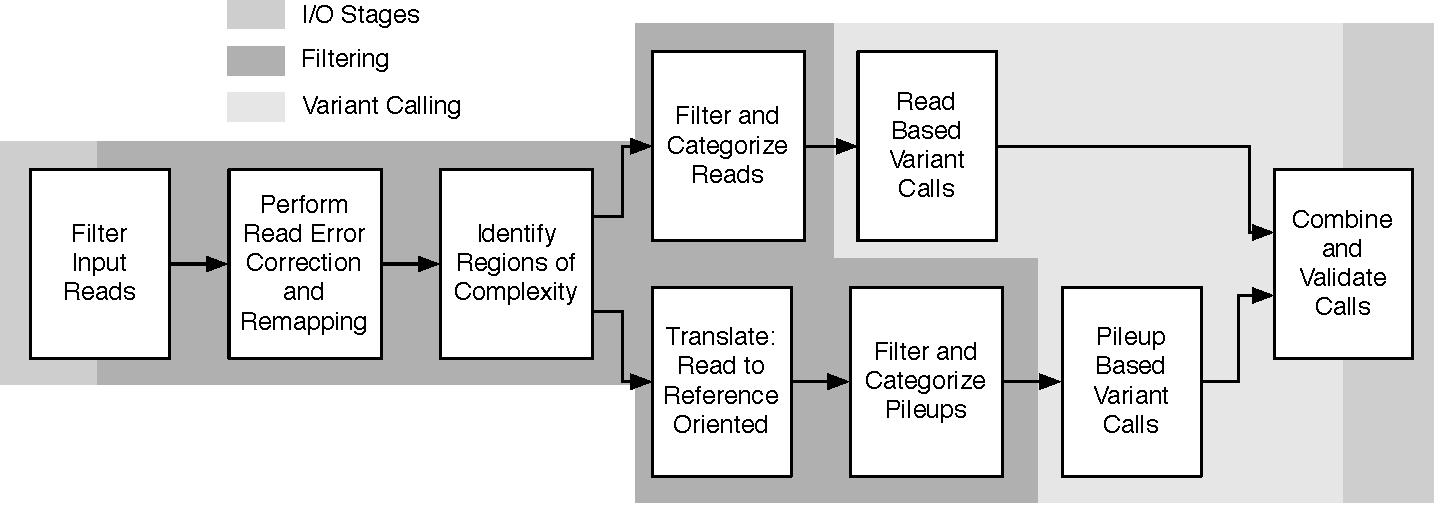
\includegraphics[width=0.9\linewidth]{avocado-architecture.pdf}
\end{center}
\caption{System Architecture}
\label{fig:architecture}
\end{figure}

\texttt{avocado} is roughly divided into four stages:

\begin{enumerate}
\item \textbf{Read pre-processing:} Applies transformations from the ADAM pipeline, including sort, duplicate marking, BQSR, and
local realignment. Operates strictly on read data.
\item \textbf{Filtering:} Selects the best algorithm for calling variants on a segment of data; transforms data to be reference-oriented
if necessary. This is discussed in~\S\ref{sec:algorithm-selection}.
\item \textbf{Variant calling:} Calls genotypes for samples in input set on either read-oriented or reference-oriented data. These
algorithms are discussed in~\S\ref{sec:local-assembly} and~\S\ref{sec:snp-calling}.
\item \textbf{Variant filtering:} Here, variant data is calculated from genotypes using the ADAM API~\cite{massie13}. Additionally,
variants can be filtered for quality.
\end{enumerate}

All stages are designed to be configurable, and easy to replace. Specifically, the filtering and variant calling stages are designed
with a specific eye towards modularity. For variant calls, we provide a base class, and two specialized subclasses for variant
calls that operate on either read or reference oriented data. A variant calling algorithm can be added by implementing one
of these class interfaces, and then registering the call with a filter. For filters, we provide two filtering stages: the first operates
on read data, and is used to implement the filter described in~\S\ref{sec:algorithm-selection}. The second filtering stage operates
on pileup~(reference oriented) data---currently, we use this to filter out pileups that have no mismatch evidence. For both of these
filters, we provide a simple interface for developers to implement.

To improve pipeline performance, we made a significant optimization to the reads-to-pileup transformation step. At the start of
transforming reads into reference oriented data, the reads are sorted by reference position. However, due to the partitioning
used by Spark~\cite{zaharia10}, after a na\"{\i}ve transformation of reads to single reference oriented bases, the reference
oriented bases are no longer sorted. This makes the ensuing grouping of bases by position very expensive due to significant disk
shuffle I/O. Instead, we perform a quasi-streaming transform on the read data. Here, the sorted read blocks are chunked together.
All of the reads in this window are then converted into pileup bases, and then grouped together into rods. This leads to significantly
better performance, but has tricky edge cases: reads that border the end of a group must be duplicated into both read groups.

\subsection{Local Assembly}
\label{sec:local-assembly}

% TODO(peter, 12/16) Peter 1pg

Given a partition of reads, we can group them by their starting locus in
intervals of $W$, creating regions of length $W+L-1$ where $L$ is the
read length.
Within each region, we can evaluate the likelihood of observing the reads
given the reference haplotype:
\begin{align}
  \mathcal L(H^\text{ref})
  &\equiv\mathbf P(\{r_i\}|H^\text{ref}) \\ \nonumber
  &=\prod_i\mathbf P(r_i|H^\text{ref})
\end{align}
where $\mathbf P(r|H)$ is obtained from aligning the read and the
candidate haplotype by a pairwise HMM alignment \cite{durbin98}.
Note that, in practice, all probabilities are computed in units of logarithm
base $10$, so products become sums, etc.

If a reference haplotype likelihood is below a fixed threshold,
the region corresponding to the haplotype is marked \emph{active}.
Each \emph{active region} is assembled independently and in parallel.
Note that our definition of an active region is similar in spirit but not in
implementation to the ``active regions'' defined by the Complete Genomics
variant caller \cite{carnevali12} and current versions of GATK \cite{depristo11}.

The assembly of an active region is a kind of $k$-mer graph or ``Eulerian''
approach \cite{pevzner01}.
We start by splitting all reads assigned to the region into $k$-mers, where $k$
is a fixed parameter for all assemblies.
A read generates $L-k+1$ total $k$-mers.
Each $k$-mer is uniquely identified by the substring of its originating read.
Because of coverage overlap and sequence repeats, some $k$-mers will be
duplicates;
these are consolidated, and the duplication factor is recorded as the
$k$-mer multiplicity.
The $k$-mers define edges in the completed $k$-mer assembly graph.
Within a read, each adjacent pair of $k$-mers have an overlapping substring of
length $k-1$;
these are seeded as the initial vertices in the $k$-mer graph.
Because there are duplicated $k$-mers, some vertices will be ``merged,''
connecting the graph.
Unlike an exact de Bruijn graph, which connects all overlaps between $k$-mers,
we only connect the overlaps found in the reads, performing a simple form of
read threading.

Once the $k$-mer graph is complete, we perform a depth-first traversal with an
upper bound on the total path multiplicity, defined as the sum of the edge
multiplicities, to enumerate a set of possible paths.
The traversal begins at a graph source, and a completed path must also end at a
sink.
Each path is an assembled haplotype to be evaluated.

From the assembled haplotypes, we order them according to the haplotype
likelihood:
\begin{align}
  \mathcal L(H_j)
  &=\prod_i\mathbf P(r_i|H_j).
\end{align}
Among the ordered haplotypes, we pick the top scoring haplotypes and ignore
the low scoring ones.
The likelihood of observing the reads $\{r_i\}$, given a pair of haplotypes
$H_j$ and $H_{j'}$, is defined to be \cite{albers11}:
\begin{align}
  \mathcal L(H_j,H_{j'})
  &\equiv\mathbf P(\{r_i\}|H_j,H_{j'}) \\ \nonumber
  &=\prod_i\left[ \frac{\mathbf P(r_i|H_j) }{2} + \frac{\mathbf P(r_i|H_{j'})}{2} \right].
\end{align}
We compute the posterior probability of observing the pair of haplotypes
$H_j$ and $H_{j'}$ from the haplotype pair likelihood and a haplotype pair
prior probability \cite{albers11}:
\begin{align}
  \mathbf P (H_j,H_{j'}|\{r_i\})&=\frac{1}{Z}\mathcal L(H_j,H_{j'})\mathbf P(H_j,H_{j'})
\end{align}
where $Z$ is a normalization:
\begin{align*}
  Z&=\sum_j\sum_{j'}\mathcal L(H_j,H_{j'})\mathbf P(H_j,H_{j'})
\end{align*}
and where we obtain the prior $\mathbf P (H_j,H_{j'})$ by aligning the haplotype
pair with the same pairwise HMM alignment as above, and taking the product of
the prior probabilities for each SNP and indel event.

We choose the maximum a priori estimate among haplotypes with any variants
as the called non-reference maternal and paternal haplotype pair \cite{albers11}:
\begin{align}
  (H_\text{mat}^\text{nonref},H_\text{pat}^\text{nonref})&=\arg\max_{H_j,H_{j'}:n_\text{var}(H_j,H_{j'})>0}\mathbf P(H_j,H_{j'}|\{r_i\}).
\end{align}
Similarly, we may define the reference haplotype pair as
$(H^\text{ref},H^\text{ref})$.
The error probability of calling the non-reference haplotype pair is:
\begin{align}
  &\mathbf P_\text{error}(H_\text{mat}^\text{nonref},H_\text{pat}^\text{nonref}) \\ \nonumber
  &=\frac{\mathbf P(H^\text{ref},H^\text{ref})}{\mathbf P(H_\text{mat}^\text{nonref},H_\text{pat}^\text{nonref})+\mathbf P(H^\text{ref},H^\text{ref})}.
\end{align}
The quality score of all variants present in the nonreference haplotype pair
is defined as the Phred scaling of $\mathbf P_\text{error}$.

\subsection{Genotype Calling}
\label{sec:snp-calling}

For one sample at a site, we can estimate the genotype likelihood based on the number of reads that match the
reference genome and the quality of each of these reads. Let the number of reads at site $a$ be $k$ and the ploidy be $m$. Without
loss of generality assume the first $l\leq k$ bases match the reference, and the rest do not. Let $\epsilon_j$ be the
error probability of the $j$th read base. We have that,
\begin{align}
\mathcal{L}(g) =& \frac{1}{m^k} \prod_{j=1}^l \left[ (m-g)\epsilon_j + g( 1 - \epsilon_j )\right] \notag\\
&\times\prod_{j=l+1}^k \left[(m-g)(1-\epsilon_j) + g\epsilon_j \right]
\label{eq:likelihood}
\end{align}

Here we are only leveraging the data of a single sample. Performance can be improved by considering statistics associated
with other samples. If a study involves sequencing many individuals from a population, it is beneficial to run them jointly in order
to determine population parameters like per-locus allele frequency spectrum (AFS) and minor allele frequency (MAF)
( \S~\ref{sec:joint-variant-calling}). However, when genotyping a single individual computational time can be saved by looking
these parameters up in a database such as dbSNP. If the population MAF at site $a$ is $\phi_a$, the likelihood can be
compensated by the prior probability of seeing a non-reference allele, and the genotype is
\begin{equation}
\hat{g}_{a} = \arg\max_g \frac{\mathcal{L}(g)P[g|\phi_a]}{\sum_g \mathcal{L}(g)P[g|\phi_a]}
\end{equation}

where $P[g|\phi] = {m\choose g} \phi^g (1-\phi)^{m-g}$ is the pmf of the binomial distribution.
% Brielin .5pg

\subsection{Joint Variant Calling}
\label{sec:joint-variant-calling}
When genotyping several individuals one may wish to genotype them jointly while determining population allele statistics,
 especially when said individuals are from a specific population of interest. In this case, we can use the EM procedure of
 Samtools Mpileup. Given the data for several individuals and using the likelihood in (\ref{eq:likelihood}), we can
 infer the population MAF per site via iteration of
 \begin{equation}
 \phi_a^{(t+1)} = \frac{1}{M}\sum_{i=1}^n\frac{g\mathcal{L}(g)P[g | \phi_a^{(t)}] }{ \sum_g \mathcal{L}(g)P[g | \phi_a^{(t)}]}
 \end{equation}
 
 where $n$ is the number of individuals, $M=\sum_{i=1}^nm_i$ is the total number of chromosomes and $P$ is the binomial
 likelihood described above. This population MAF can then be used in genotyping as above. 

% Brielin .5pg

\subsection{Algorithm Selection}
\label{sec:algorithm-selection}

% Frank .5pg

As discussed in~\S\ref{sec:architecture}, we seek to improve the performance of our variant caller without reducing accuracy by directing
the variant caller to use higher accuracy methods in areas that show increased complexity. Loosely, we define a complex region as an
area that is highly similar to other areas of the genome, or where it is likely that a complex variant~(such as an indel) is segregating. To
identify those regions, we use the following heuristics:

\begin{itemize}
\item Areas that are highly similar to other areas of the genome can be distinguished by low mapping quality. Reduced mapping quality
indicates that alignment found several areas where the read could map with similar quality.
\item Complex variants lead to a change in coverage over the effected area. Deletions will see reduced coverage, and insertions lead
to increased coverage.
\end{itemize}

We implemented our filter by stepping a window across the reference genome. The window was stepped by 1000 base pairs. In each
1000 base pair window, we would compute the average coverage, and mapping quality. If a window violated either of the mapping
quality or the coverage threshold, we would flag it as high complexity and pass it to the assembler. If a window did not violate either
of those two thresholds, we built pileups out of the data on this interval, and then used the genotyping methods described
in~\S\ref{sec:snp-calling}.

We provided several tuning parameters to the end user. Specifically, the end user could set the target mapping quality and coverage
deviation percentage~(percent change from mean coverage). Table~\ref{tab:filter} summarizes the sensitivity of these parameters.

\begin{table}[h]
\caption{\% Reads in High Complexity Region}
\begin{center}
\begin{tabular}{| c || c | c | c |}
\hline
\bf MapQ,Cov & \bf 0.2 & \bf 0.4 & \bf 0.6 \\
\hline
\hline
\bf 40 & 88\% & 54\% & 20\% \\
\bf 50 & 90\% & 56\% & 22\% \\
\bf 60 & 98\% & 91\% & 88\% \\
\hline 
\end{tabular}
\end{center}
\label{tab:filter}
\end{table}

As can be noted, mapping complexity begins to saturate as the mapping quality threshold increases to 60\footnote{Phred-scaled 60 is
equivalent to a probability of $P=0.999999$ that the read is correctly mapped.}, and as the coverage variation coefficient decreases to 0.2.

\section{Evaluation}
\label{sec:evaluation}

% Frank 0.5pg

\subsection{Accuracy}
\label{sec:accuracy}

% Frank 1pg

\subsection{Performance}
\label{sec:performance}

% Frank 1pg

\section{Future Work}
\label{sec:future-work}

% Frank 1pg

Since assembly depends on the exact sequences of the input data, the quality of
the reads is critical for performing an accurate assembly.
One error correction method is spectral filtering \cite{pevzner01}, which depends
on the observation that the distribution of $k$-mers from all reads with respect to
multiplicity is bimodal, one due to the Poisson sampling of reads (with high
multiplicity), the other due to errors (with low multiplicity), so that splitting
the reads between the two modes and keeping the reads near the mode with higher
multiplicity serves to prune the poor quality reads.
%Errors in the read data lead to \emph{spurs}, which are spurious short sections
%of the graph connected to the source or the sink. % todo cite for spurs?
%We do not remove spurs, although it may slightly improve performance.
Empirically, we have found during other work that utilizing mate pair
information greatly improves the quality of an assembly. % todo how to cite this?
We also do not employ mate pair threading, which requires collecting the
insert size distribution of the data, but we expect that implementing it has
the potential to vastly improve the accuracy of variant calls.

\section{Conclusion}
\label{sec:conclusion}

\appendix

\section{Availability}
\label{sec:availability}

\texttt{avocado} is open source and is licensed under the Apache 2 license. The source code is available at:

\url{http://www.github.com/bigdatagenomics/avocado}

\section{Genotype/Variant Refactoring}
\label{sec:genotype-variant-refactoring}

Traditionally, variant calling has involved genotyping $n$ samples, and then determining which of the genotypes of these samples
contain true variants. This involves the calculation of a \textit{variant quality} score\footnote{Loosely defined as the likelihood that
there is \emph{at least} one genotype with this variant out of all haplotypes seen in the call set.}, and filtering variants.

Semantically, all of the information necessary for the creation of variant data can be extracted from the genotypes of the samples.
Therefore, the step of packing/unpacking genotype data to create variant calls is unnecessary. To reduce the likelihood of making
errors, we have migrated code to do this into the ADAM~\cite{massie13} framework. Then, to get variant calls, we must just genotype
the samples we see, and call the ADAM library.

This does not preclude joint variant calling---although joint variant calling implies that multi-sample data is being used to influence
the filtering of variants, this is a bit of a misnomer. Practically, as discussed in~\S\ref{sec:joint-variant-calling}, joint variant calling
involves the use of data from multiple samples to refine genotype probabilities across a population to support genotypes that are
frequently seen in this population.

%
% The following two commands are all you need in the
% initial runs of your .tex file to
% produce the bibliography for the citations in your paper.
\bibliographystyle{abbrv}
\bibliography{avocado-cs262-report}  

\balancecolumns
% That's all folks!
\end{document}
